\documentclass{article}
\usepackage[utf8]{inputenc}
\usepackage{amsmath}
\usepackage{xcolor}
\usepackage[top=2cm, bottom=2cm, left=2cm, right=2cm]{geometry}
\setlength\parindent{0pt}

\usepackage{listings}
%\usepackage{color}
\usepackage{graphicx}
\usepackage{float}
\usepackage{caption}

\usepackage{verbatim}
\let\oldv\verbatim
\let\oldendv\endverbatim

%\userpackage{minted}

\definecolor{dkgreen}{rgb}{0,0.6,0}
\definecolor{gray}{rgb}{0.5,0.5,0.5}
\definecolor{mauve}{rgb}{0.58,0,0.82}
\definecolor{light-gray}{gray}{0.95}


\lstset{frame=tb,
  language=Java,
  aboveskip=6mm,
  belowskip=6mm,
  showstringspaces=false,
  columns=flexible,
  basicstyle={\small\ttfamily},
  numbers=none,
  numberstyle=\tiny\color{gray},
  keywordstyle=\color{blue},
  commentstyle=\color{dkgreen},
  stringstyle=\color{mauve},
  breaklines=true,
  breakatwhitespace=true,
  tabsize=3,
  backgroundcolor=\color{light-gray},
  language=Matlab
}

%\usepackage{natbib} replaced by line below to make refernces work
\usepackage[square,sort,comma,numbers]{natbib}
\usepackage[nottoc,numbib]{tocbibind} %to get references in table of contants
\usepackage{graphicx}

\usepackage{bm}

\usepackage{hyperref}
\hypersetup{
	colorlinks,
	citecolor=black,
	filecolor=black,
	linkcolor=black,
	urlcolor=black
}

\usepackage{mdframed}
\usepackage{lipsum} % for creating dummy text
\mdfdefinestyle{MyFrame}{%
	linecolor=black,	
	backgroundcolor=gray!20!white,
	skipbelow = 8mm,
	skipabove = 8mm}

\usepackage{scrextend}

\usepackage{multimedia}
\usepackage{media9}

\title{Fys4150\\Project 3\\ }
\author{Peter Killingstad and Karl Jacobsen\\
\\
\url{https://github.com/kaaja/fys4150}}
\begin{document}
	
\maketitle



\section*{Note to instructurs about Github repository}
If the above Github-link does not work, it is eighter because you have not yet accepted our invite to the repository, or you have not yet provided us with an e-mail adress available at Github so that we can invite you. The Github user you will be invited from is "kaaja". If the latter applies to you, please send us an e-mail with an e-mailadress available in Github or your Github username so that we can send you an invite. Our e-mailadresses: peter.killingstad@hotmail.com, karljaco@gmail.com.



\section*{Abstract}


\section{Introduction}

\section{Theory}

\subsection{Physics}
Derive equations, scaling.

\subsection{Programming}
Motivate classes. 



\section{Results}
Short overview: our class program. Scenarios

\subsection{Class implementation}
How we did it.

\subsection{Forward Euler versus Velocity Verlet}
The below figures show the results for the x and y-positions as functions of time, forward Euler to the left and Velocity Verlet to the right. 


\begin{minipage}{.49\textwidth} 
	\begin{figure}[H]
		\centering
		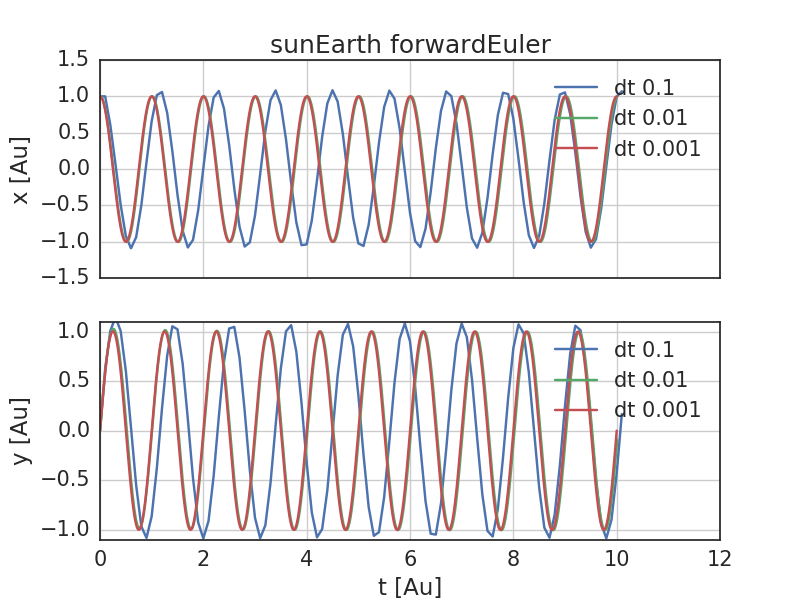
\includegraphics[width=0.99\textwidth]{/home/karl/doc/subj/att/fys4150/project3/resultsKeep/plots/sunEarthTimesForwardEuler.png}
		\caption{Sun-Earth system. Effect of $\Delta t$ over a 10 year period. \\ \textit{The Forward Euler method seems to converge for the two smallest $\Delta t$}}
		\label{1}
	\end{figure}
\end{minipage}\hfill
\begin{minipage}{.49\textwidth} 
	\begin{figure}[H]
		\centering
		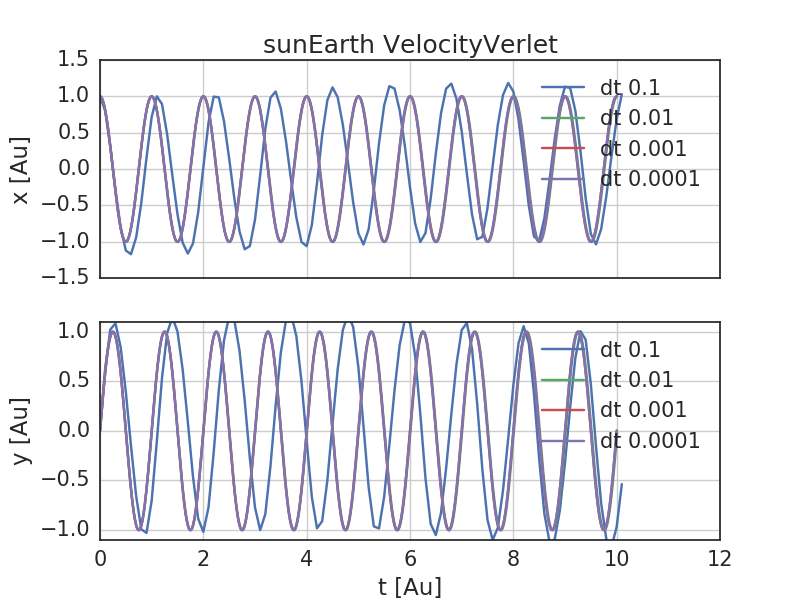
\includegraphics[width=0.99\textwidth]{/home/karl/doc/subj/att/fys4150/project3/resultsKeep/plots/sunEarthTimesVelocityVerlet.png}
		\caption{Sun-Earth system. Effect of $\Delta t$ over a 10 year period. \\ \textit{The Velocity verlet method seems to converge faster than Forward Euler}}
		\label{1}
	\end{figure}
\end{minipage}\hfill
\vspace{2ex}

As can be seen of the figures above, both methods converges when $\Delta t$ is lowered.  Also the Velocity Verlet method seems to converge faster.\\

The next two sets of figures shows the orbits for different $\Delta t$ for the two methods.

\begin{minipage}{.49\textwidth} 
	\begin{figure}[H]
		\centering
		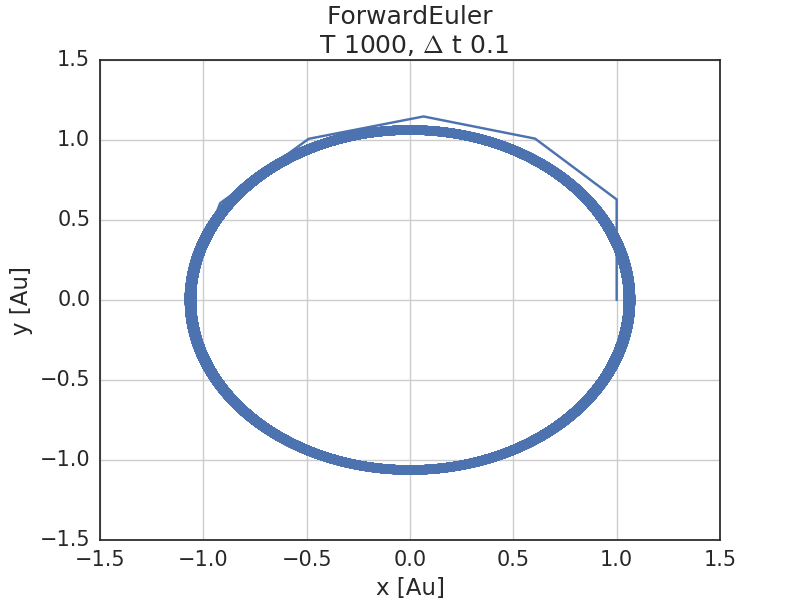
\includegraphics[width=0.99\textwidth]{/home/karl/doc/subj/att/fys4150/project3/resultsKeep/plots/sunEarthfinalTime1000N100000ForwardEuler.png}
		\caption{Sun-Earth system. Forward Euler. 1 000 years \\ \textit{Non-circulat orbits when time step is large.}}
		\label{1}
	\end{figure}
\end{minipage}\hfill
\begin{minipage}{.49\textwidth} 
	\begin{figure}[H]
		\centering
		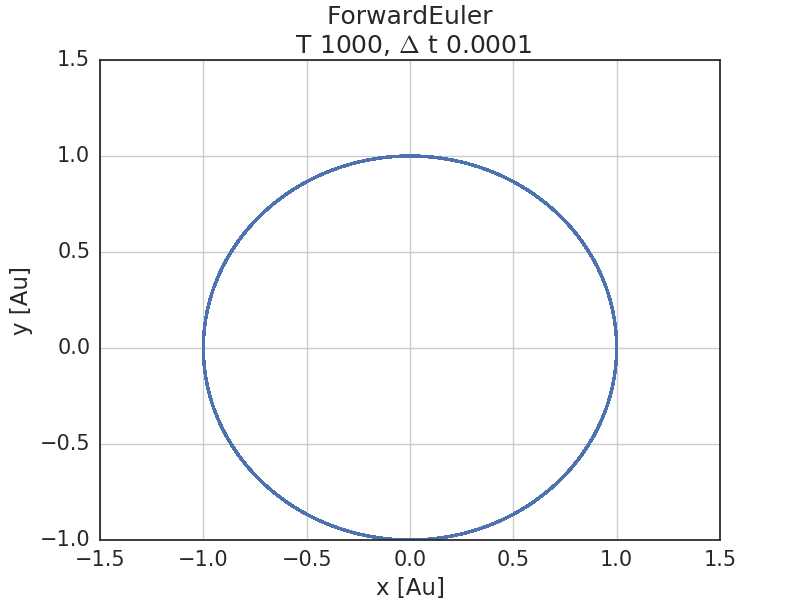
\includegraphics[width=0.99\textwidth]{/home/karl/doc/subj/att/fys4150/project3/resultsKeep/plots/sunEarthfinalTime1000N100000000ForwardEuler.png}
		\caption{Sun-Earth system. Forward Euler. 1 000 years. \\ \textit{For $\Delta t = 0.0001$, the forward Euler seems to give circular orbits, but we can see that the solution changes.}}
		\label{1}
	\end{figure}
\end{minipage}\hfill
\vspace{2ex}



\begin{minipage}{.49\textwidth} 
	\begin{figure}[H]
		\centering
		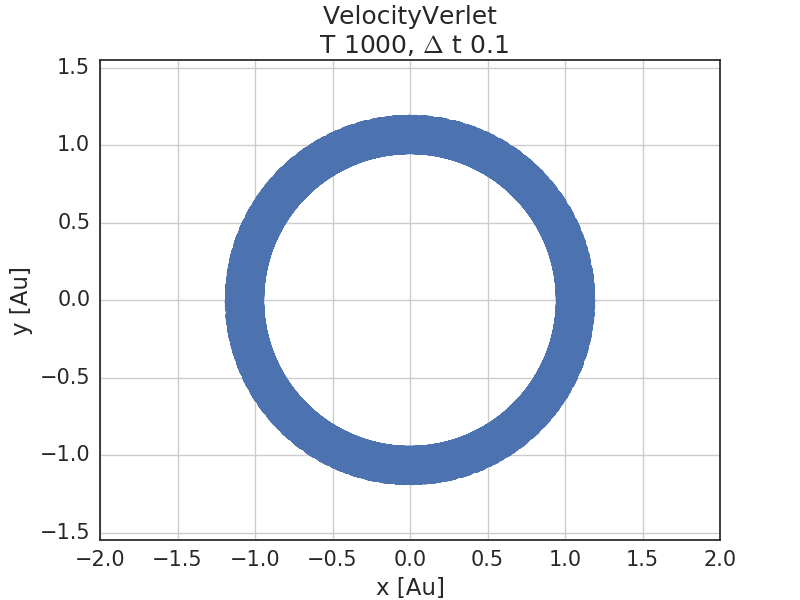
\includegraphics[width=0.99\textwidth]{/home/karl/doc/subj/att/fys4150/project3/resultsKeep/plots/sunEarthfinalTime1000N10000VelocityVerlet.png}
		\caption{Sun-Earth system. Velocity Verlet. 1000 years. \\ \textit{Large time step gives bad solutions also for Velocity Verlet.}}
		\label{1}
	\end{figure}
\end{minipage}\hfill
\begin{minipage}{.49\textwidth} 
	\begin{figure}[H]
		\centering
		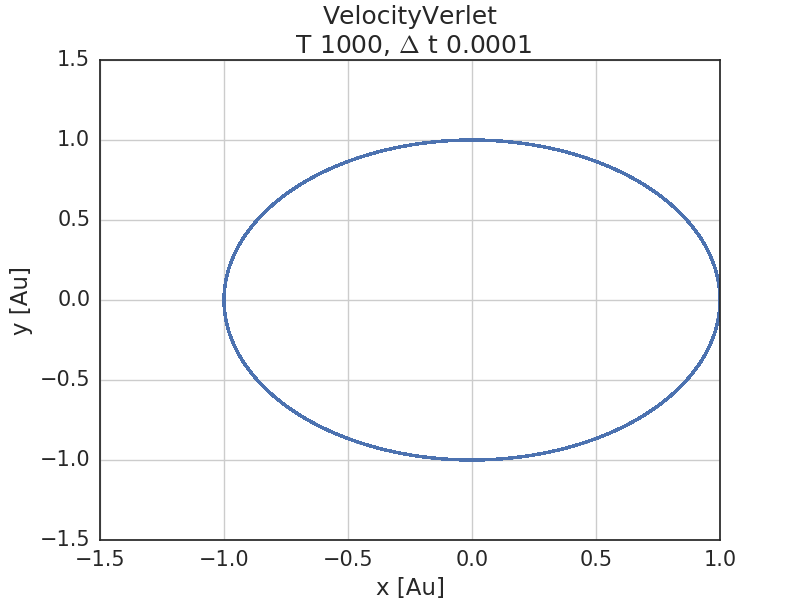
\includegraphics[width=0.99\textwidth]{/home/karl/doc/subj/att/fys4150/project3/resultsKeep/plots/sunEarthfinalTime1000N100000000VelocityVerlet.png}
		\caption{Sun-Earth system. Velocity Verlet. 1 000 years. \\ \textit{Compare to Forward Euler}}
		\label{1}
	\end{figure}
\end{minipage}\hfill
\vspace{2ex}

The 2 sets of figures above confirms what we found in the figures with x and y-position agains time: The precision is bettered when $\Delta t$ is lowered. \\

DO: Explain why energy and angular momentum are preserved.\\

The below figures show the difference in total energy compared to the initial total energy, forward Euler to the left and Velocity Verlet to the right.


\begin{minipage}{.49\textwidth} 
	\begin{figure}[H]
		\centering
		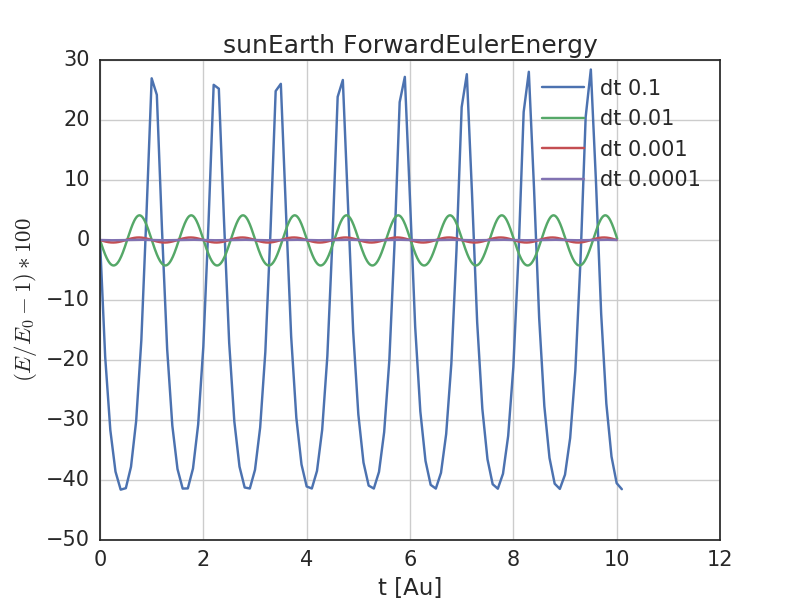
\includegraphics[width=0.99\textwidth]{/home/karl/doc/subj/att/fys4150/project3/resultsKeep/plots/sunEarthEnergyForwardEuler.png}
		\caption{Sun-Earth system. Total Energy divided by total energy first time step. Forward Euler. 10 years. \\ \textit{Energy is not preserved with the Forward Euler method}}
		\label{1}
	\end{figure}
\end{minipage}\hfill
\begin{minipage}{.49\textwidth} 
	\begin{figure}[H]
		\centering
		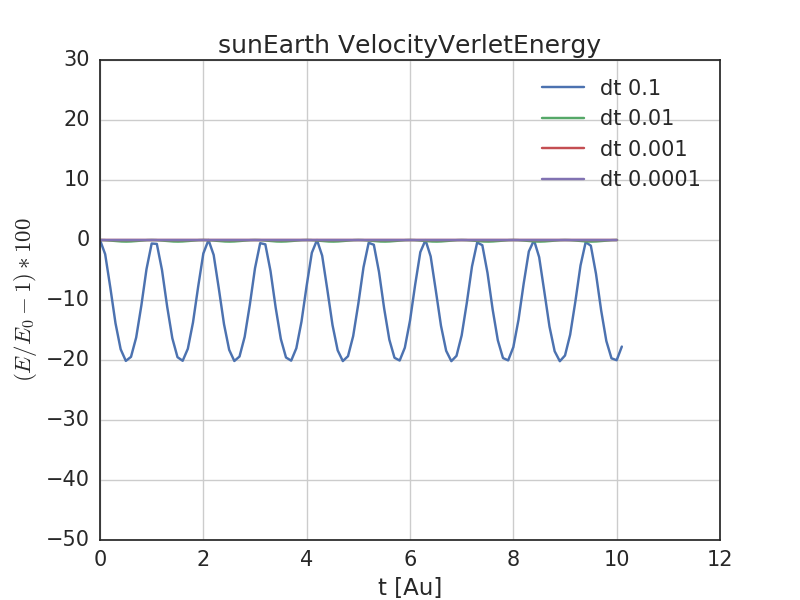
\includegraphics[width=0.99\textwidth]{/home/karl/doc/subj/att/fys4150/project3/resultsKeep/plots/sunEarthEnergyVelocityVerlet.png}
		\caption{Sun-Earth system. Total Energy divided by total energy first time step. Velocity Verlet. 10 years. \\ \textit{Energy is preserved in Velocity Verlet provided fine enough time step. }}
		\label{1}
	\end{figure}
\end{minipage}\hfill
\vspace{2ex}

The two figures above show that for forward Euler, energy can actually increase, even for smaller $\Delta t$. For Velocity Verlet, energy seems to be preserved faster compared to Forward Euler. Also, Velocity Verlet never make energy, as is the case for Forward Euler.\\

The next figure shows the same kind of figures as for energy above, but now for angular momentum. DO: Write why angular momentum is preserved.



\begin{minipage}{.49\textwidth} 
	\begin{figure}[H]
		\centering
		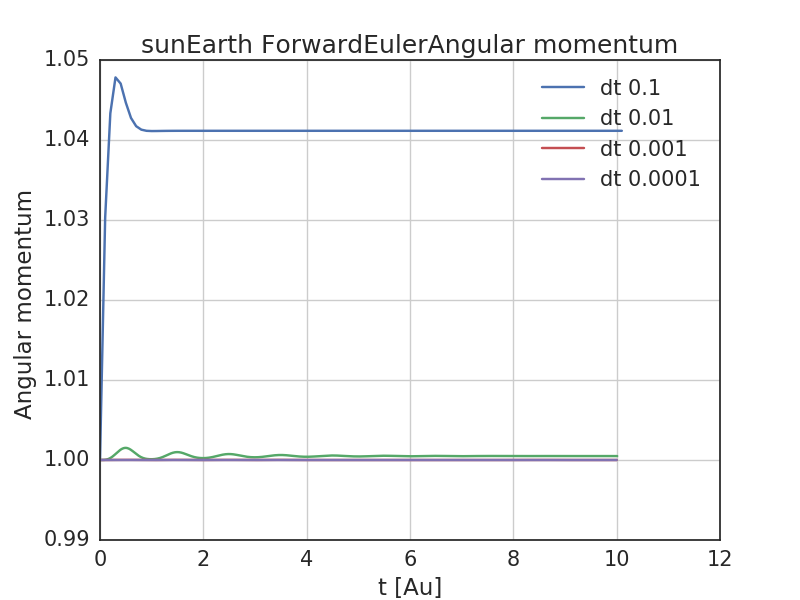
\includegraphics[width=0.99\textwidth]{/home/karl/doc/subj/att/fys4150/project3/resultsKeep/plots/sunEarthAngularMomentumForwardEuler.png}
		\caption{Sun-Earth system. Angular momentum divided by angular momentum first time step. Forward Euler. 10 years. \\ \textit{Angular momentum seems to be conserverd for the finest time step.}}
		\label{1}
	\end{figure}
\end{minipage}\hfill
\begin{minipage}{.49\textwidth} 
	\begin{figure}[H]
		\centering
		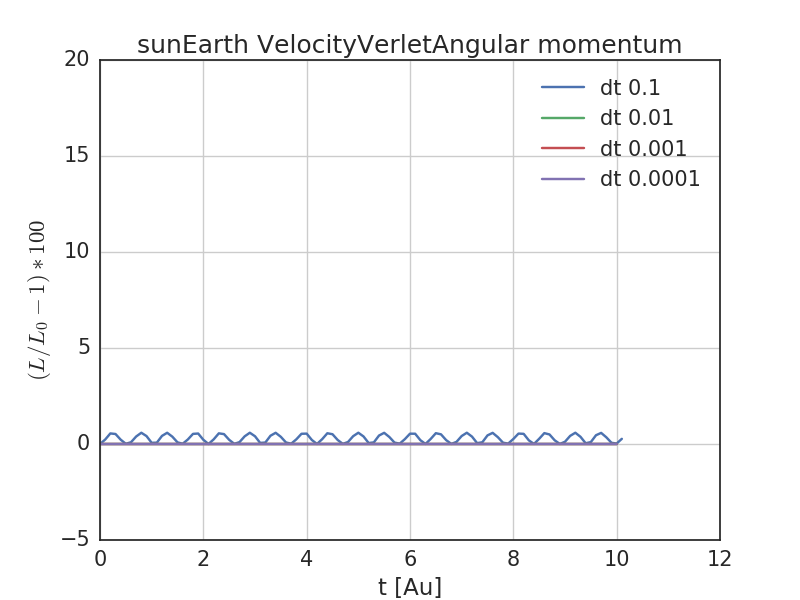
\includegraphics[width=0.99\textwidth]{/home/karl/doc/subj/att/fys4150/project3/resultsKeep/plots/sunEarthAngularMomentumVelocityVerlet.png}
		\caption{Sun-Earth system. Angular momentum divided by angular momentum first time step. Velocity Verlet. 10 years. \\ \textit{Angular momentum is conserverd given suffiently fine time steps. Conservation achieved faster than with Forward Euler.}}
		\label{1}
	\end{figure}
\end{minipage}\hfill
\vspace{2ex}

The figures above show that as $\delta t$ gets low, angular momentum is preserved. ALso, Velocity Verlet seems to give good angular momentum approximations compared to Forward Euler.\\

Since we know the exact solution for energy and angular momentum, or more precisely, the exact solution for the change, we have constructed a norm measure for computing convergence rates of the schemes. The error-norm is the supremum of the largest difference in energy compared to initial energy. The below figures show the results. DO: Write what to expect of these norms. We have truncation estimate for velocity and position, so it should just be to insert this into energy equation.

\begin{minipage}{.49\textwidth} 
	\begin{figure}[H]
		\centering
		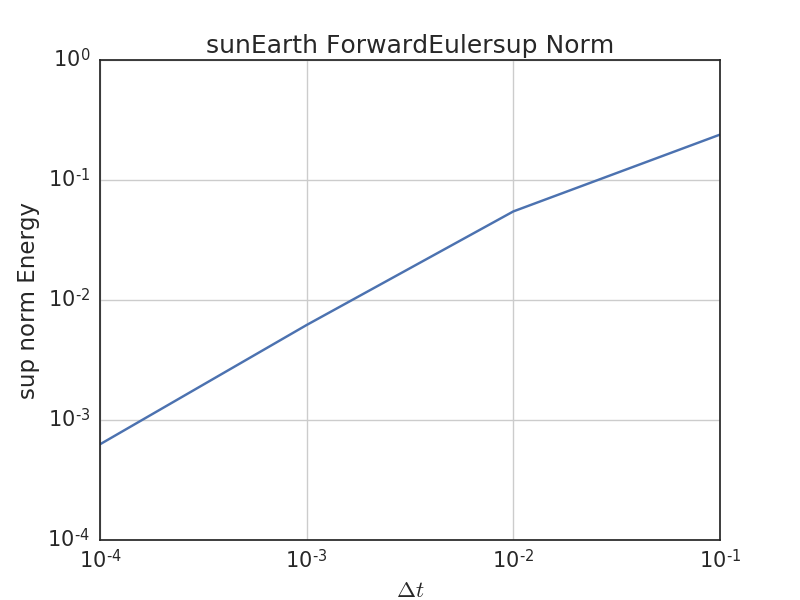
\includegraphics[width=0.99\textwidth]{/home/karl/doc/subj/att/fys4150/project3/resultsKeep/plots/sunEarthsupNormForwardEuler.png}
		\caption{Sun-Earth system. Sup-norm total energy. Forward Euler. \\ \textit{Forward Euler's sup-norm goes like $\mathcal{O}(\Delta t)$}}
		\label{1}
	\end{figure}
\end{minipage}\hfill
\begin{minipage}{.49\textwidth} 
	\begin{figure}[H]
		\centering
		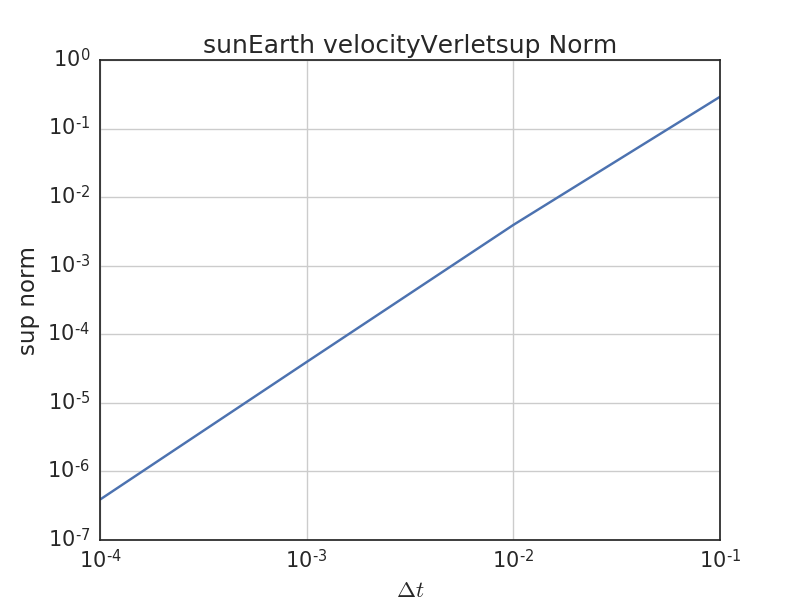
\includegraphics[width=0.99\textwidth]{/home/karl/doc/subj/att/fys4150/project3/resultsKeep/plots/sunEarthsupNormVelocityVerlet.png}
		\caption{Sun-Earth system. Sup-norm total energy. Velocity Verlet \\ \textit{The sup-norm in energy for Velocity Verlet goes one higher order than Forward Euler}}
		\label{1}
	\end{figure}
\end{minipage}\hfill
\vspace{2ex}

The above two figures shows that the error goes as 1st order for Forward Euler, while Velocity Verlet goes like 2nd order. DO: How does this compare to expectations?\\

In the same manner as for the energy-norms above, we have also constructed a norm for angular momentum. DO: What to expect. The below figure displays the results for the angular momentum norms.

\begin{minipage}{.49\textwidth} 
	\begin{figure}[H]
		\centering
		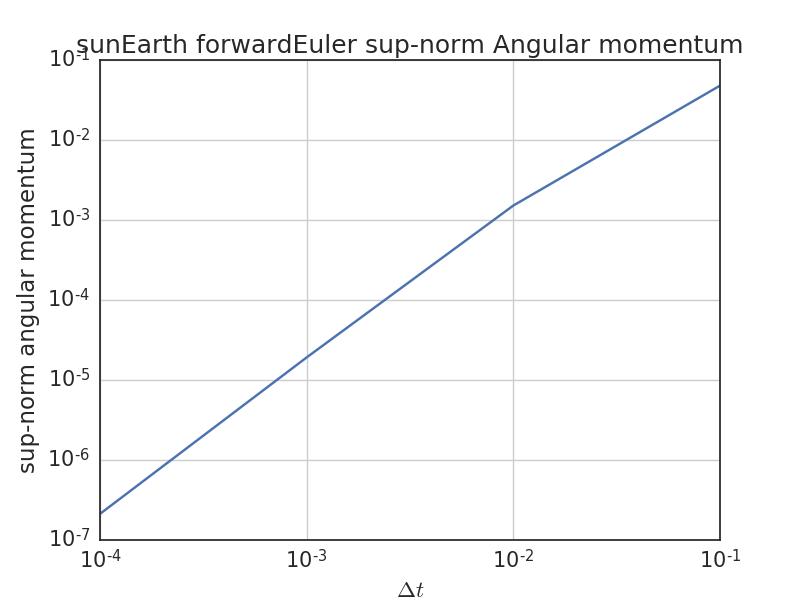
\includegraphics[width=0.99\textwidth]{/home/karl/doc/subj/att/fys4150/project3/resultsKeep/plots/sunEarthsupNormAngularMomentumForwardEuler.png}
		\caption{Sun-Earth system. Sup-norm Angular Momentum. Forward Euler \\ \textit{Forward Euler's sup-norm for angular momentum goes like $\mathcal{O}(\Delta t^2)$}.}
		\label{1}
	\end{figure}
\end{minipage}\hfill
\begin{minipage}{.49\textwidth} 
	\begin{figure}[H]
		\centering
		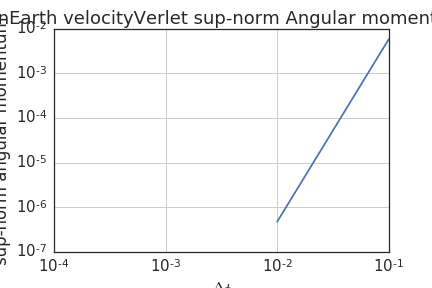
\includegraphics[width=0.99\textwidth]{/home/karl/doc/subj/att/fys4150/project3/resultsKeep/plots/sunEarthsupNormAngularMomentumVelocityVerlet.png}
		\caption{Sun-Earth system. Sup-norm Angular momentum. Velocity Verlet \\ \textit{Velocity Verlet's sup-norm error less than $10^{-12}$ like $\mathcal{O}(\Delta t^4)$.}}
		\label{1}
	\end{figure}
\end{minipage}\hfill
\vspace{2ex}

The two figures above shows that also for angular momentum, the order of the error-norm is higher for Velocity Verlet compared to Forward Euler, but now the difference is of order two. Also we see that the orders are doubled from the energy norms. DO: Comment on why higher order than energy, and how the results compare to expectations.\\

Knowledge about a methods correctness, discussed above, is crucial, but efficiency is also important. DO: FLOP-count for Forward-Euler and Velocity Verlet. The below figures show the computation time for the methods, forard Euler to the left and Velocity Verlet to the right.

\begin{minipage}{.49\textwidth} 
	\begin{figure}[H]
		\centering
		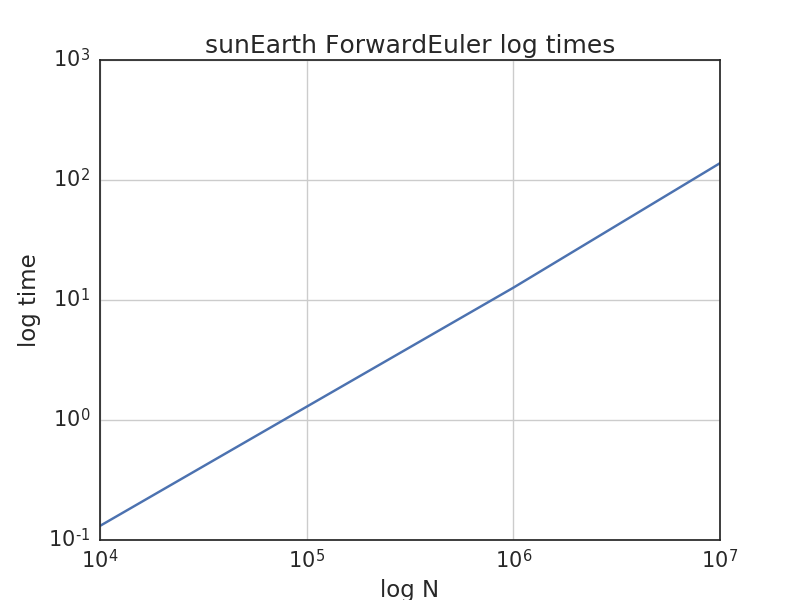
\includegraphics[width=0.99\textwidth]{/home/karl/doc/subj/att/fys4150/project3/resultsKeep/plots/sunEarthlogTimeUsedForwardEuler.png}
		\caption{Sun-Earth system. Log time. Forward Euler \\ \textit{Forward Euler's $\mathcal{O}(N)$}.}
		\label{1}
	\end{figure}
\end{minipage}\hfill
\begin{minipage}{.49\textwidth} 
	\begin{figure}[H]
		\centering
		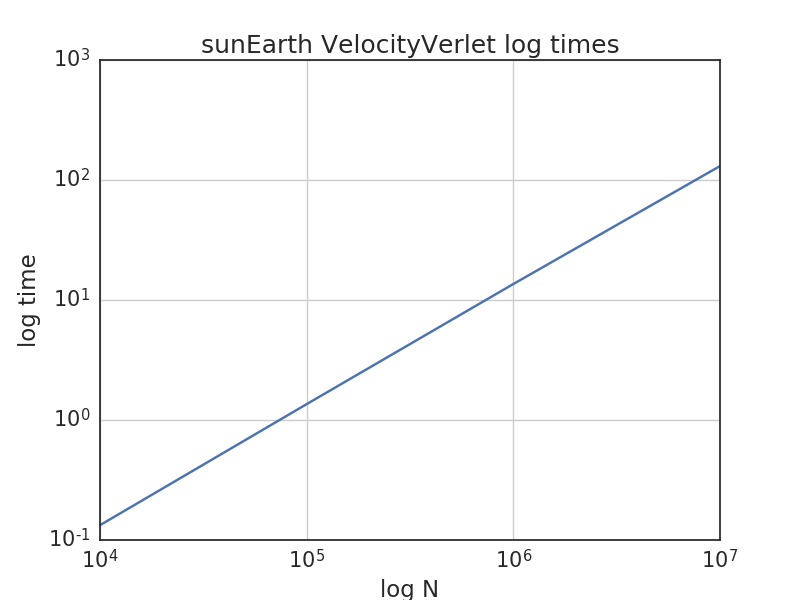
\includegraphics[width=0.99\textwidth]{/home/karl/doc/subj/att/fys4150/project3/resultsKeep/plots/sunEarthlogTimeUsedVelocityVerlet.png}
		\caption{Sun-Earth system. Log time. Velocity Verlet \\ \textit{Velocity Verlet's log time is of the same order as Forward Euler.}}
		\label{1}
	\end{figure}
\end{minipage}\hfill
\vspace{2ex}

The two figures above show that the Forward Euler and the Velocity Verlet method both has solution times that is of order 1 in N. This is as expected. The difference in FLOPS between forward Euler and Velocity Verlet is...DO.


\subsection{Escape velocity}
Another test to see if the solver obeys the physical laws, is to check if the escape velocity is correct. The escape velcoity equals the velcoity where potential energy equals kinetic energy

\begin{subequations}
	\begin{align}
	E_k  &= E_p \\
	\frac{1}{2} m_E v_{Escape}^2&= \frac{G M_{Sun} M_E}{r_0}\\
	\rightarrow v_E&=\sqrt{\frac{2G M_{Sun} }{r_0}}\\
	&=\sqrt{\frac{2* 4 \pi^2 AU^3 }{AU yr^2}}\\
	&=2 \pi\sqrt{2}\frac{ AU }{yr}
	\end{align}
\end{subequations}

Based on the above equation, we expect the simulations to gove escape then $v > 2\pi \sqrt{2}$. The figures below show the results.

\begin{figure}[H]
	\centering
	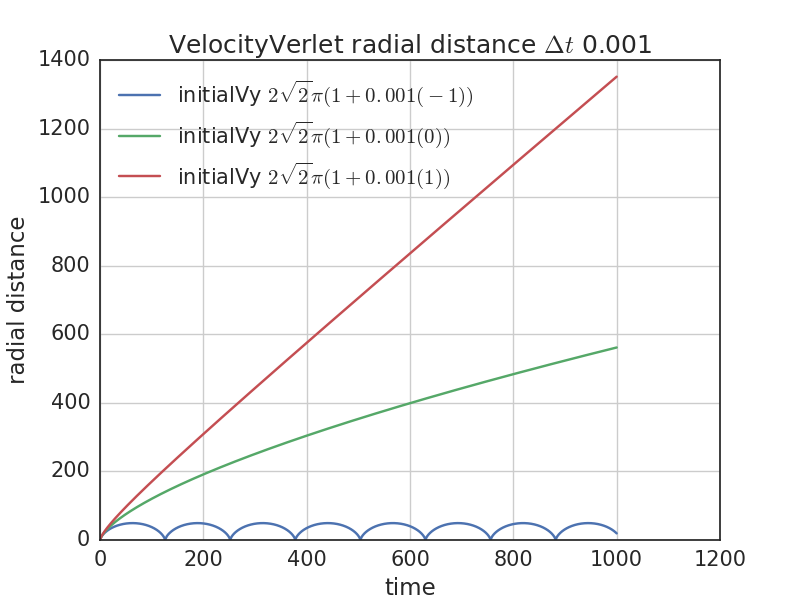
\includegraphics[width=0.99\textwidth]{/home/karl/doc/subj/att/fys4150/project3/resultsKeep/plots/sunEarthTerminalVelocityradialDistanceVelocityVerlet.png}
	\caption{Sun-Earth system. Escape valocity. Radial distance earth sun. \\ \textit{$v = 2\sqrt{2}\pi$ is an ustable equilibrium.}}
	\label{1}
\end{figure}



\begin{minipage}{.33\textwidth} 
	\begin{figure}[H]
		\centering
		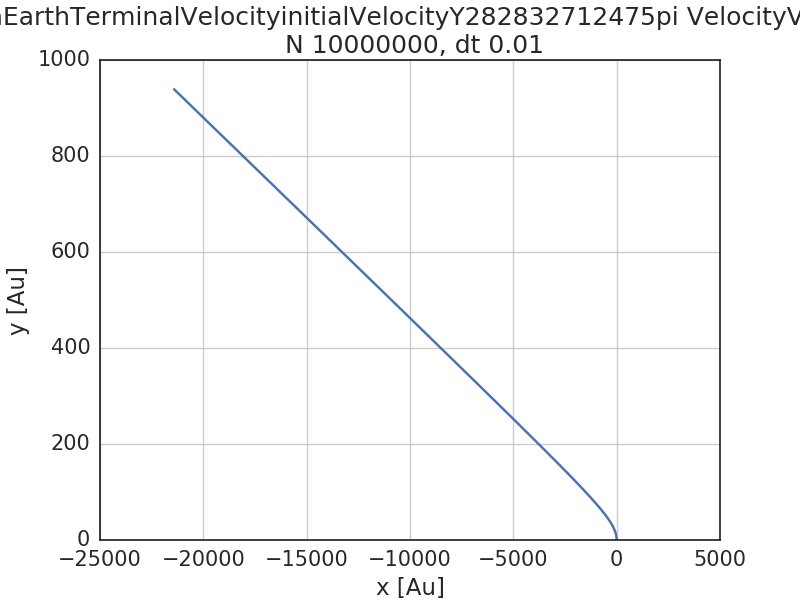
\includegraphics[width=0.99\textwidth]{/home/karl/doc/subj/att/fys4150/project3/resultsKeep/plots/sunEarthTerminalVelocityinitialVelocityY1piVelocityVerlet.png}
		\caption{Sun-Earth system. Escape valocity. Orbits. \\ \textit{No escape for $v < 2/sqrt{2} \pi$}}
		\label{1}
	\end{figure}
\end{minipage}\hfill
\begin{minipage}{.33\textwidth} 
	\begin{figure}[H]
		\centering
		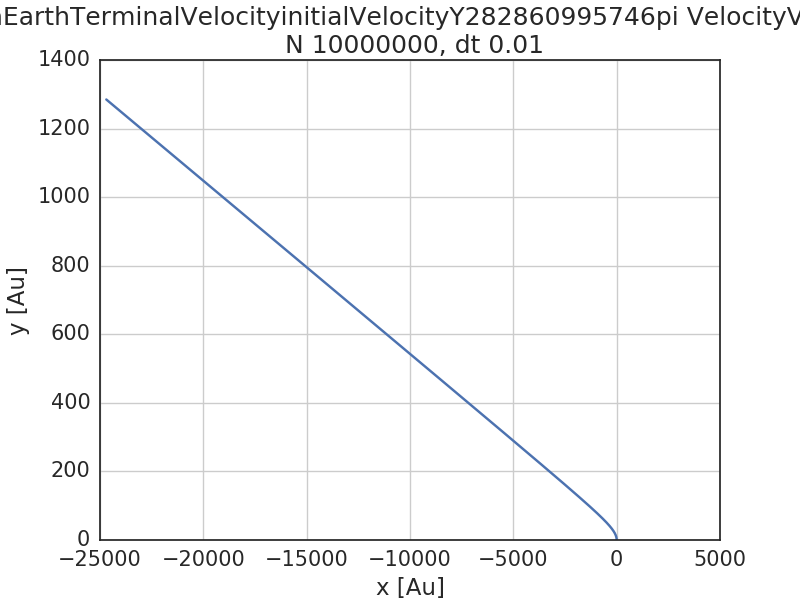
\includegraphics[width=0.99\textwidth]{/home/karl/doc/subj/att/fys4150/project3/resultsKeep/plots/sunEarthTerminalVelocityinitialVelocityY2piVelocityVerlet.png}
		\caption{Sun-Earth system. Escape valocity. Orbits. \\ \textit{No escape for $v = 2/sqrt{2} \pi$}}
		\label{1}
	\end{figure}
\end{minipage}\hfill
\begin{minipage}{.33\textwidth} 
	\begin{figure}[H]
		\centering
		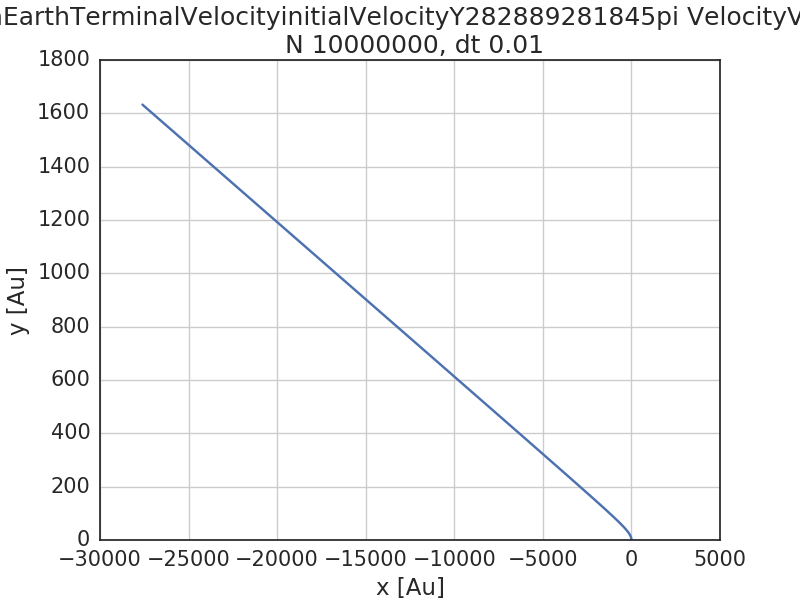
\includegraphics[width=0.99\textwidth]{/home/karl/doc/subj/att/fys4150/project3/resultsKeep/plots/sunEarthTerminalVelocityinitialVelocityY3piVelocityVerlet.png}
		\caption{Sun-Earth system. Escape valocity. Orbits. \\ \textit{Escape for $v < 2/sqrt{2} \pi$}}
		\label{1}
	\end{figure}
\end{minipage}\hfill
\vspace{2ex}

The figures above show that the simulated escape velocity is very close to the exact terminal velcocity, $2 \pi \sqrt{2}$, supporting the previous results indicating the validity of our solver as a good approximation method.\\

Another test, to see if the numerical solutions corresponds to analytical solutions, is to simulate the two planet system with different gravitational forces. DO: Write down a more general formula for the kinetic energy based on the revised forces.\\

The below figures show escapce velocities for the three different gravitational forces, all forces being lower than the standard force simulated above.


\begin{minipage}{.3\textwidth} 
	\begin{figure}[H]
		\centering
		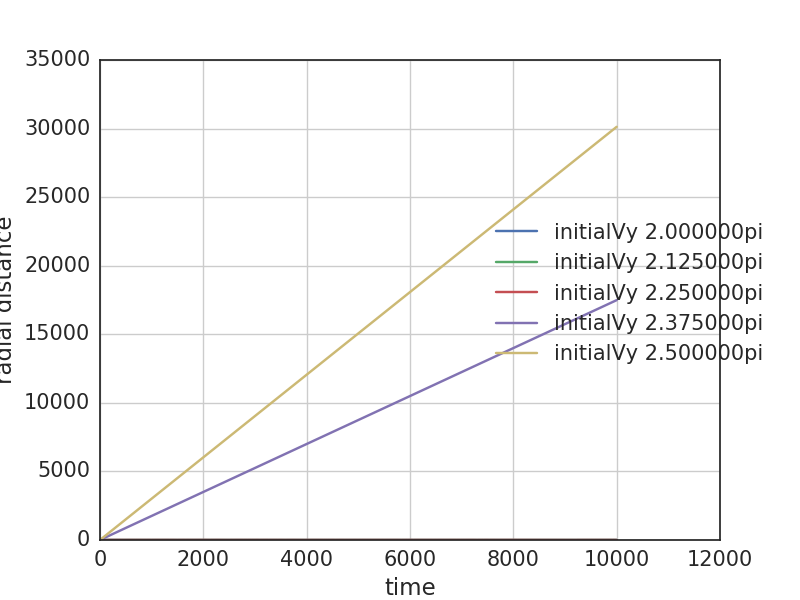
\includegraphics[width=0.99\textwidth]{/home/karl/doc/subj/att/fys4150/project3/resultsKeep/plots/sunEarthradialDistanceAlternativeForcebeta35.png}
		\caption{Sun-Earth system. Alternative force. Escape valocity. $\beta = 2.5$ \\ \textit{Escape velocity is reduced compared to case with normal gravititation.}}
		\label{1}
	\end{figure}
\end{minipage}\hfill
\begin{minipage}{.3\textwidth} 
	\begin{figure}[H]
		\centering
		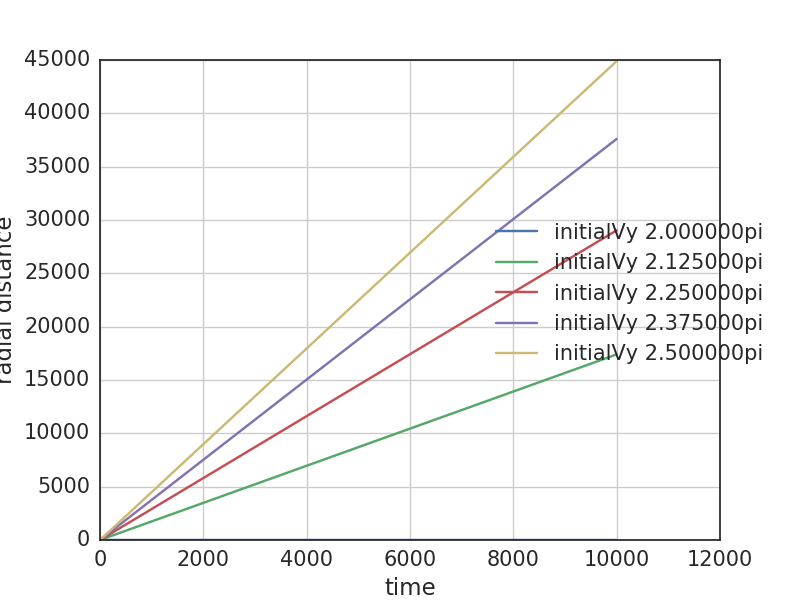
\includegraphics[width=0.99\textwidth]{/home/karl/doc/subj/att/fys4150/project3/resultsKeep/plots/sunEarthradialDistanceAlternativeForcebeta39.png}
		\caption{Sun-Earth system. Alternative force. Escape valocity. $\beta = 2.9$ \\ \textit{The escape velocity is further reduced, and seems to be closer to $2  \pi$}}
		\label{1}
	\end{figure}
\end{minipage}\hfill
\begin{minipage}{.3\textwidth} 
	\begin{figure}[H]
		\centering
		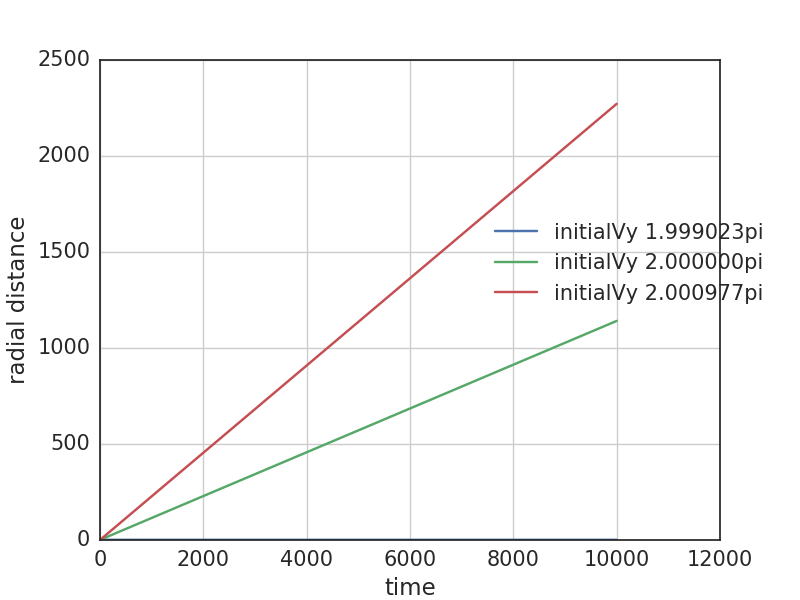
\includegraphics[width=0.99\textwidth]{/home/karl/doc/subj/att/fys4150/project3/resultsKeep/plots/sunEarthradialDistanceAlternativeForcebeta40.png}
		\caption{Sun-Earth system. Alternative force. Escape valocity. $\beta = 3.0$ \\ \textit{We get escape at $v = 2\pi$.}}
		\label{1}
	\end{figure}
\end{minipage}\hfill
\vspace{2ex}

The figures above show that the escape velocities are lowered when the gravitational forces are lowered. DO: Check agains thoretical expression. We see from the right most figure that the escape velocity is the same as the exact. DO: check the previous claim.

\subsection{Three planets}
Above we have seen that the solvers correspond well with expected behavoiur: Forward Euler does not preserve energy, while Velocity Verlet does, and basic exact results for escapce velocities, energy and angular momentum is well approximated. However, the above was only tested on a two-object system. To check whether the solver works for multibody systems, with more than two objects, a third planet, Jupiter, is added.\\

The figure below shows the orbits of the three body-system.

DO: Create and insert figures for 3 body non-moving sun here.\\

The figures above shows that the solver produces reasonable results for the three body system also. As for two bodies, the largest $\delta t$'s give bad approximations, while the smaller $\Delta t$'s give good approximations. DO: check the previous claim.\\

\subsection{Center of mass system}
All the above simulations were based on the assumption that the sun was stationary. This is not the case in reality. To make the  solver more realistic, we now introduce movement in the sun by letting the sun be modelled just as the other planets, gravity affecting also the sun's movement. \\

To make the plots easy to interpret, we make sure that the center of mass of the system is stationary. This we do by adjusting the initial velocity of the sun, utilizing the fact that the angular momentum of the system is preserved

\begin{subequations}
	\begin{align}
	0 &= \frac{d \vec R}{dt}	\\
	&= \frac{d}{dt} (\frac{1}{M} \sum_i^{Planets+Sun} m_i \vec{v}_i)\\
	&= \frac{1}{M} \sum_i^{Planets+Sun} m_i v_i \\
	\rightarrow 0 &=m_{sun} \vec{v}_{sun} + \sum_i^{Planets} m_i \vec{v}_i \\
	\vec{v}_{Sun} &= - \frac{\sum_i^{Planets} m_i \vec{v}_i}{m_{Sun}}
	\end{align}
\end{subequations}

The below figure shows the results with a moveing sun.\\

DO: Insert figure with moving sun and normal Jupiter mass here.\\

The figure above shows that the result of including movement in the sun is small. DO: Check the previous claim. To see how the program deals with a moving sun, we increase the mass of Jupiter. This should increase the movement of the sun, and make the results in the moving sun case different from the results in the stationary sun case. The results are shown in the figures below.\\

DO: Insert figures with increased mass of Jupiter, both for moving and non-moving sun.\\

The figures above show that when Jupiter's mass in increased, there is a signifiacant effect of introducing movement in the sun. The last figure also clearly shows that the center of mass remains fixed.


\subsection{Solar system}

\subsection{Perihelion precession}

\section{Conclusions}

\section{Feedback}
\subsection{Project 1}
This project has been extremely educational. We learned about about c++, especially pointers and dynamic memory allocoation. Also which for us was a well forgotten subject, we learned about dangerous of numerical round-off errors. \\

We feel the size of the project is large, much larger than typical assignments in other courses. However, the quality and quantity of the teaching without a doubt made the workload managable. The detailed lectures, combined with the fast and good respones on Piazza helped a lot!\\

We think the project could have gone even smoother, if we on the 2nd lab-session had learned basic branching in Github. We used a considerable amount of time finding out of this.\\

All in all, two thumbs up!

\subsection{Project 2}
\begin{itemize}
	\item  catch: We ended up using a lot of time making this work properly. Still we have some problems with catch and Qt. We think we might had benefited from a demonstration at the lab.
	
	\item We were not able to understand the revised Sturm-Bisection algorithm from Barth et al.'s \cite{barth} paper on the revised Sturm-Bisection. 
	
	\item Apart from the small details above, we are very happy about this project. How would have thought linear algebra could be fun?!
\end{itemize}

\subsection{Project 3}
\begin{itemize}
	\item  Classes: Very useful!
\end{itemize}













\pagebreak
\begin{thebibliography}{9}
	\bibitem{barth} 
	Barth, Martin, Wilkinson (1967)
	Calculation of eigenvalues of a symmetric tridiagonal matrix by the method of bisection. \textit{Numeriche mathematik 9, 386 - 393 (1967)}
	
	\bibitem{MHJ} 
	Hjorth-Jensen, M.(2015)
	Computational physics. Lectures fall 2015. 
	\url{https://github.com/CompPhysics/ComputationalPhysics/tree/master/doc/Lectures}
	
	\bibitem{MHJProject2} 
	Hjorth-Jensen, M.(2017)
	Project 2, fys4150 2017.
	\url{https://github.com/CompPhysics/ComputationalPhysics/blob/master/doc/Projects/2017/Project2/pdf/Project2.pdf}
	
	\bibitem{kiusalaas} 
	Kiusalaas, J.(2013)
	Numerical Methods in Engineering with Python 3. 3rd edition.
	
	\bibitem{taut} 
	Taut, M. (1993)
	Two electrons in an external oscillator potential: Particular analytic solutions of a Coulomb correlation problem \textit{Phys. Rev. A 48, 3561 (1993).}
	
	


\end{thebibliography}


\end{document}
